\documentclass{beamer}
\usepackage{xcolor}
\usepackage{lmodern}
\usepackage{xspace}
%\usepackage[frozencache=true,cachedir=minted-cache]{minted}
\usepackage{minted}
\usepackage{tikz}
\usepackage{pgfplots}

\newcommand{\argot}{\texttt{ArGoT}\xspace}
\newcommand{\isa}{\texttt{IS-A}\xspace}

\newminted{xml}{fontsize=\tiny, 
                   frame=lines,
                   framesep=3mm}

\addtobeamertemplate{title page}{\includegraphics[scale=.05]{{University_of_Pittsburgh_seal.png}} \hfill 
\includegraphics[scale=.3]{fabstracts2.png}}{}

\title{\argot: arXiv Glossary of Terms}
%\title{\texttt{ArGoT}: A Glossary of Terms from the arXiv}
%\subtitle{A comprehensive dictionary   of all mathematical lexicon}
\author{Luis Berlioz\\
\texttt{lab232@pitt.edu}}
\institute{University of Pittsburgh}

\begin{document}

\defverbatim[colored]\exampleCode{
    \begin{xmlcode}
<definition index="8">
<stmnt> A sequence _inline_math_ of non-zero vectors in a Banach space _inline_math_ is said to be 
a Schauder basic sequence if it is a Schauder basis of its closed linear span (see _citation_). 
This is equivalent to say that there exists a constant _inline_math_ such that for every _inline_math_ 
with _inline_math_ and every _inline_math_ we have (1) _display_math_ The least constant _inline_math_ 
for which inequality () holds is called the basis constant of _inline_math_. A Schauder basic sequence 
_inline_math_ is said to be monotone if _inline_math_. It is said to be seminormalized 
(respectively normalized) if there exists _inline_math_ such that _inline_math_ 
(respectively _inline_math_) for every _inline_math_. </stmnt>
<dfndum>Schauder basic sequence</dfndum>
<dfndum>basis constant</dfndum>
<dfndum>Schauder basic sequence</dfndum>
<dfndum>seminormalized</dfndum></definition>
    \end{xmlcode}
}

%%%%  FRAME  %%%%
\begin{frame}
    \maketitle
\end{frame}

%%%%  FRAME  %%%%
\begin{frame}
    \frametitle{\argot in a few words...}
    \begin{itemize}
        \item Database of \emph{definitions} and \emph{terms} extracted from the arXiv using machine learning.
            \pause
        \item 350,000 mathematical terms.
            \pause
        \item Two versions: Neural Networks (NN) and Supp. Vector Machines and Stoch. Grad. Descent (SGD)
            \pause
        \item Compare to graph datasets:  \textcolor{red}{CS PhDs Relationships} and \textcolor{brown}{WordNet}.
            \pause
        \item Two examples using the arXiv metadata and Hyperbolic word embeddings.
    \end{itemize}
\end{frame}

%%%%  FRAME  %%%%
\begin{frame}
    \frametitle{Example of a database entry}
    An example from: \structure{arxiv.org/abs/0805.2034}
    \begin{center}
        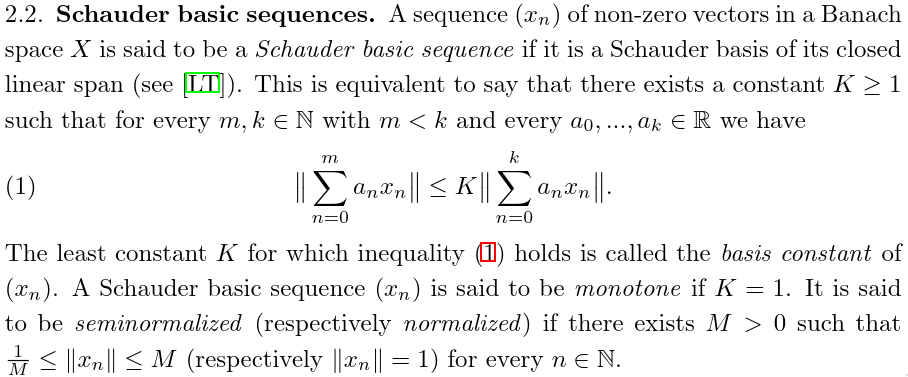
\includegraphics[width=0.8\textwidth]{def2.png}
    \end{center}
    \pause
    \exampleCode
\end{frame}


%%%%  FRAME  %%%%
\begin{frame}
    \frametitle{\argot by the numbers}
    \begin{center}
        
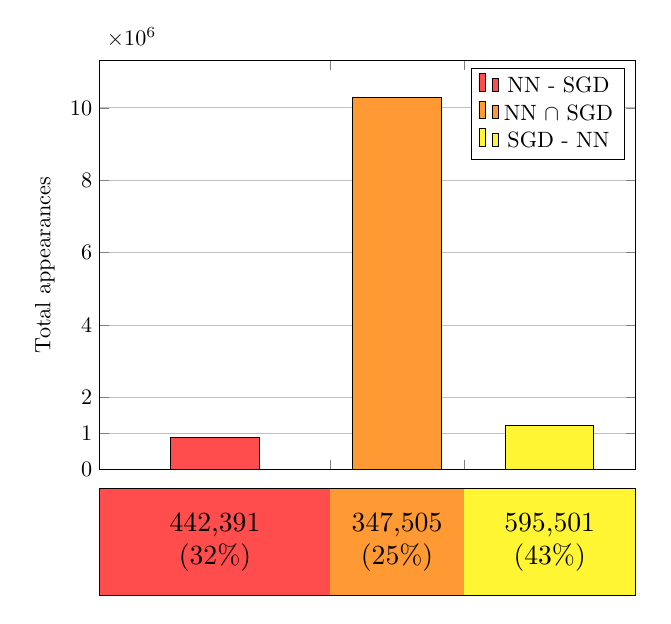
\begin{tikzpicture}[scale=0.8]
\def\mainwidth{8.5}
\def\MW{\mainwidth}
\pgfplotsset{width=\mainwidth cm, height=6.5cm, compat=1.3}

\def\NNx{.43}
\def\NN{\NNx*\mainwidth}

\def\Intx{0.25}
\def\Int{\Intx*\mainwidth}

\def\SGDx{0.32}
\def\SGD{\SGDx*\mainwidth}

\def\boxHeighta{-0.3}
\def\boxHeightb{-2}
\def\boxcc{\boxHeighta/2+\boxHeightb/2}

\tikzset{NN style/.style={ fill=red!70, mark=none} }
\tikzset{Int style/.style={ fill=orange!80, mark=none} }
\tikzset{SGD style/.style={ fill=yellow!80, mark=none} }

\begin{axis}[
xmax=1.0, xmin=0,
ymin=0.0, 
scale only axis,
bar width=40,
bar shift=0,
ybar legend,
xtick={ \NNx, \NNx+\Intx, \NNx+\Intx+\SGDx },
xticklabels={ , , },
extra y ticks={1000000.0},
extra y tick labels={1},
ymajorgrids,
%scaled y ticks=manual:{$\times 10^6$}{1000000},
scaled y ticks=real:1000000,
ytick scale label code/.code={$\times 10^6$},
%title=Unique terms vrs. Terms with repetitions,
ylabel={Total appearances},
]
\addplot+[ybar, style=NN style, draw=black] plot coordinates { (\NNx/2,881616) };
\addplot+[ybar, style=Int style, draw=black] plot coordinates { (\NNx +\Intx/2,10286789) };
\addplot+[ybar, style=SGD style, draw=black] plot coordinates { (\SGDx/2+\Intx+ \NNx,1210995) };

\legend{NN - SGD,NN $\cap$ SGD, SGD - NN}

\end{axis}
\draw[style=NN style, draw opacity=0.0] (0,\boxHeighta) rectangle (\NN, \boxHeightb);
\draw[style=Int style, draw opacity=0.0] (\NN, \boxHeighta) rectangle (\NN+\Int, \boxHeightb);
\draw[style=SGD style, draw opacity=0.0] (\NN+\Int, \boxHeighta) rectangle (\SGD+\Int+\NN, \boxHeightb);
\draw[draw] (0, \boxHeighta) rectangle (\SGD+\Int+\NN, \boxHeightb);

\node[align=center] (NNc) at (\NN/2, \boxcc) {442,391\\(32\%)};
\node[align=center] (Intc) at (\NN+\Int/2, \boxcc) {347,505\\ (25\%)} ;
\node[align=center] (SGDc) at (\NN+\Int+\SGD/2, \boxcc) {595,501\\ (43\%)};

\end{tikzpicture}

\end{center}
\end{frame}

%%%%  FRAME  %%%%
%\begin{frame}
%    \frametitle{Where the data comes from}
%    \begin{itemize}
%        \item The arXiv bulk download \structure{https://arxiv.org/help/bulk\_data}
%    \begin{center}
%        
\includegraphics[width=0.8\textwidth]{bulk1.png}
%    \end{center}
%                \pause
%            \item  \alert{LaTeXML} was used to preprocess the raw \LaTeX{} from the arXiv. 
%    \begin{center}
%        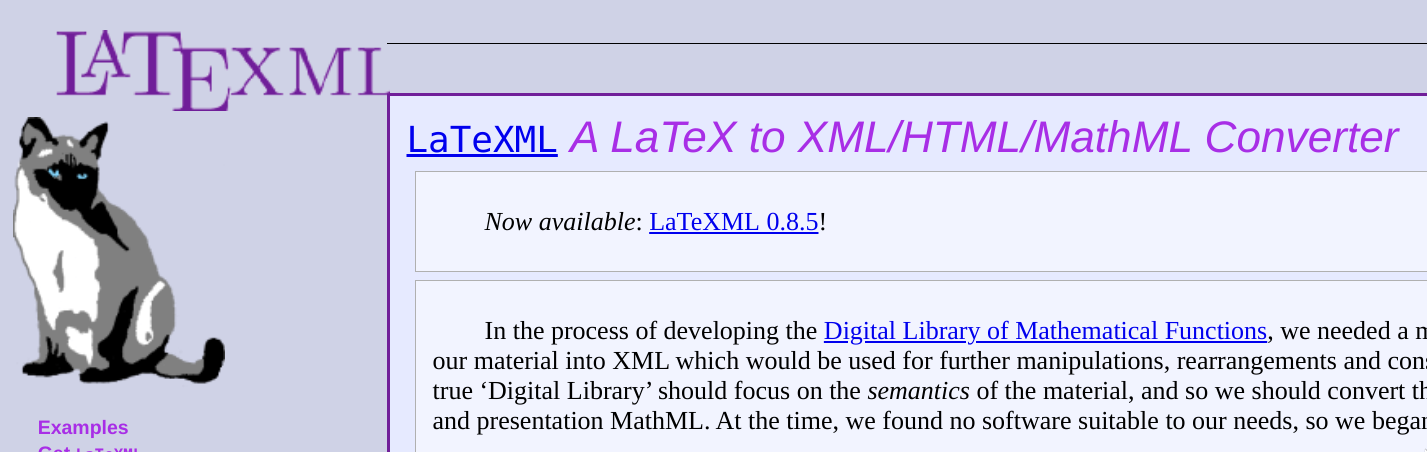
\includegraphics[width=0.8\textwidth]{latexml1.png}
%    \end{center}
%    \end{itemize}
%\end{frame}


%%%%  FRAME  %%%%
\begin{frame}
    \frametitle{Where can you find the data}
    \argot is available at: \structure{https://gl.kwarc.info/SIGMathLing/dataset-arxiv-argot-2021}
    \begin{center}
        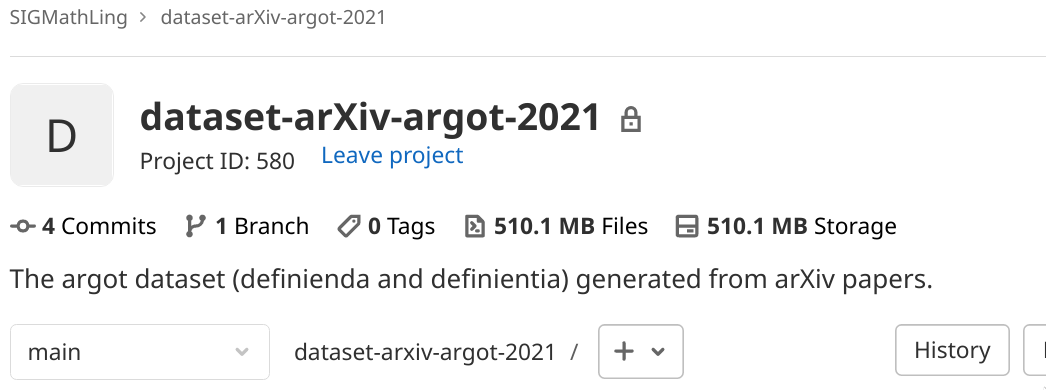
\includegraphics[width=0.8\textwidth]{download1.png}
    \end{center}

\end{frame}

%%%%  FRAME  %%%%
\begin{frame}
    \frametitle{First Example: word2vec/GloVe embeddings}
    \framesubtitle{Terms in the same field cluster together}
    \begin{center}
        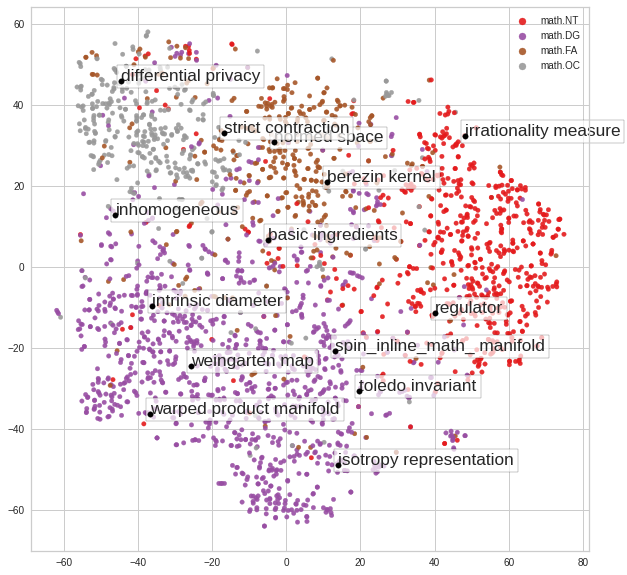
\includegraphics[width=0.8\textwidth]{../scatter_plot/scatter_option5_light.png}
    \end{center}
\end{frame}

%%%%  FRAME  %%%%
\begin{frame}
    \frametitle{Second Example: Hyperbolic Word Embeddings}
    \begin{center}
    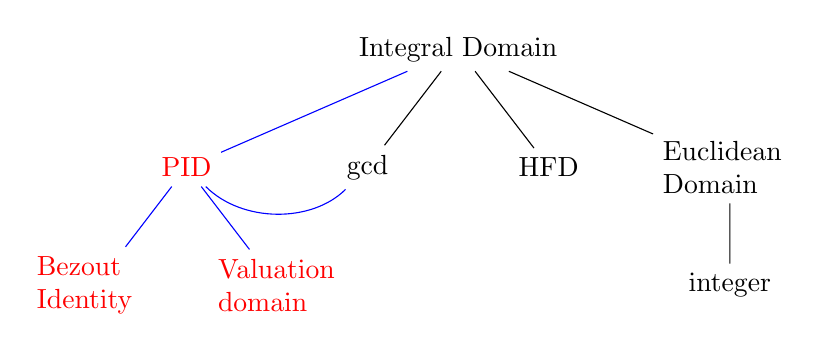
\begin{tikzpicture}

\node {Integral Domain} [sibling distance = 2.3cm, level distance = 1.5cm]
    child {[red] node (P) [fill=white] {PID} 
       child {node [text width=1.5cm]{Bezout Identity}}
       child {node [text width=1.5cm]{Valuation domain}}
    edge from parent [blue] }
    child {node (G) {gcd}}
    child {node {HFD}}
    child {node [text width=1.7cm] {Euclidean Domain}
    child {node {integer}}
    edge from parent };
\draw [blue] (P) .. controls ++(315:1) and ++(225:1) .. (G);
 
\end{tikzpicture}
\end{center}
    \begin{itemize}
        \item Approximate graph-distance in continuous space.
            \pause
        \item Identify Hypernyms, and generate a knowledge graph (KG).
    \end{itemize}
\end{frame}

%%%%  FRAME  %%%%
\begin{frame}
    \frametitle{Query results sorted by \isa score}
    \framesubtitle{Poincaré GloVe: Hyperbolic Word Embeddings}
\begin{table}
    \small
\centering
\begin{tabular}{ll|ll}
    \hline \textbf{Term} &  \isa &  
    \textbf{Term} &  \isa \\ \hline
    hyperbolic\_metric & -1.11 &  &\\
euclidean\_metric & -0.59  & digraph & -0.51 \\
metrics & -0.58 & undirected\_graph & -0.35 \\
riemannian\_metric & -0.46  &  undirected & -0.20 \\
riemannian & -0.42  & \textbf{directed\_graph} &  0.0\\
riemannian\_manif & -0.40 & graph & 1.24 \\
curvature & -0.27  & & \\
\textbf{metric} & 0.0 & & \\
\hline
banach\_algebra & -1.11  & probability\_distr & -0.24 \\
normed\_space & -0.98 & \textbf{random\_variable} & 0.0 \\
banach\_spaces & -0.38 & expectation & 0.23 \\
banach & -0.29  & distribution & 0.46 \\
closed\_subspace & -0.25 & probability & 0.67 \\
\textbf{banach\_space} & 0.0 & & \\
norm & 0.79 & & \\

\end{tabular}
\end{table}
\end{frame}

%%%%  FRAME  %%%%
\begin{frame}
    \frametitle{Wrapping Up...}
    \begin{itemize}
        \item \argot is an extensive collection of mathematical terms.
            \pause
        \item Captures the semantics of a term.
            \pause
        \item Freely available from \structure{https://gl.kwarc.info/SIGMathLing/dataset-arxiv-argot-2021}
    \end{itemize}
\end{frame}

%%%%  FRAME  %%%%
\begin{frame}
    \maketitle
\end{frame}
\end{document}

